% Fig1.tex — Onym data and metadata flow
% Standalone wrapper for IEEE submission. Identical TikZ to the inline
% figure in onym-ieee.tex; this file produces Fig1.pdf for separate upload
% to the IEEE Author Portal as the figure source asset.
\documentclass[border=4pt,tikz]{standalone}
\usepackage{amsmath,amssymb}
\usepackage{tikz}
\usetikzlibrary{positioning,arrows.meta,calc}

% Math shortcuts (mirror onym-ieee.tex)
\newcommand{\Cold}{C_{\mathsf{old}}}
\newcommand{\Cnew}{C_{\mathsf{new}}}
\newcommand{\eold}{\epsilon_{\mathsf{old}}}

\begin{document}
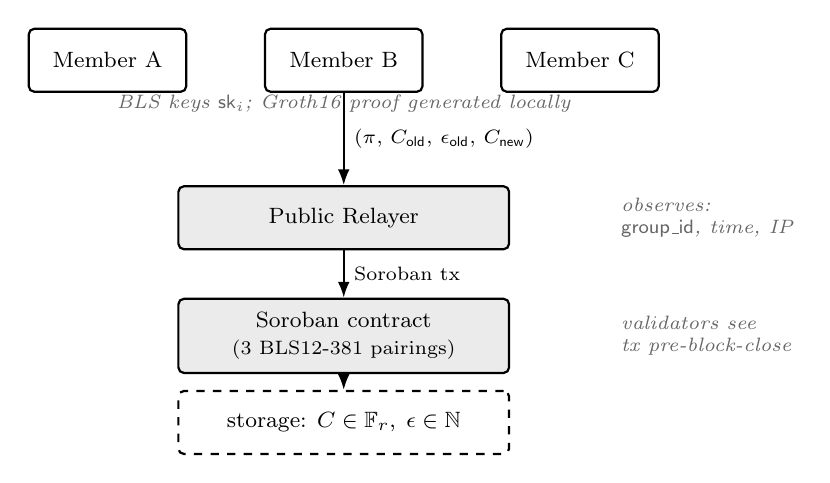
\begin{tikzpicture}[
    font=\footnotesize,
    box/.style={draw, thick, rounded corners=2pt, inner sep=5pt, align=center, minimum height=8mm},
    arr/.style={-{Latex[length=2mm]}, thick},
    leak/.style={font=\scriptsize\itshape, color=black!60, align=left}
]

% Members
\node[box, minimum width=20mm] (mA) at (-3,0) {Member A};
\node[box, minimum width=20mm] (mB) at (0,0) {Member B};
\node[box, minimum width=20mm] (mC) at (3,0) {Member C};
\node[font=\scriptsize\itshape, color=black!60] at (0,-0.55) {BLS keys $\mathsf{sk}_i$; Groth16 proof generated locally};

% Relayer
\node[box, fill=black!8, minimum width=42mm] (relay) at (0,-2.0) {Public Relayer};
\node[leak, anchor=west] at (3.4,-2.0) {observes:\\$\mathsf{group\_id}$, time, IP};

% Contract
\node[box, fill=black!8, minimum width=42mm] (chain) at (0,-3.5) {Soroban contract\\\scriptsize (3 BLS12-381 pairings)};
\node[leak, anchor=west] at (3.4,-3.5) {validators see\\tx pre-block-close};

% Storage
\node[box, dashed, minimum width=42mm] (store) at (0,-4.6) {storage: $C \in \mathbb{F}_r,\; \epsilon \in \mathbb{N}$};

% Arrows
\draw[arr] (mB.south) -- node[right, font=\scriptsize] {$(\pi,\, \Cold,\, \eold,\, \Cnew)$} (relay.north);
\draw[arr] (relay.south) -- node[right, font=\scriptsize] {Soroban tx} (chain.north);
\draw[arr] (chain.south) -- (store.north);

\end{tikzpicture}
\end{document}
